\RequirePackage{luatex85}
\documentclass[tikz]{standalone}
% Default preamble
\usepackage{pgfplots}
\pgfplotsset{compat=newest}
\usepgfplotslibrary{groupplots}
\usepgfplotslibrary{polar}
\usepgfplotslibrary{smithchart}
\usepgfplotslibrary{statistics}
\usepgfplotslibrary{dateplot}
\usepgfplotslibrary{ternary}
\usepackage[T1]{fontenc}
\usepackage{lmodern}
\begin{document}
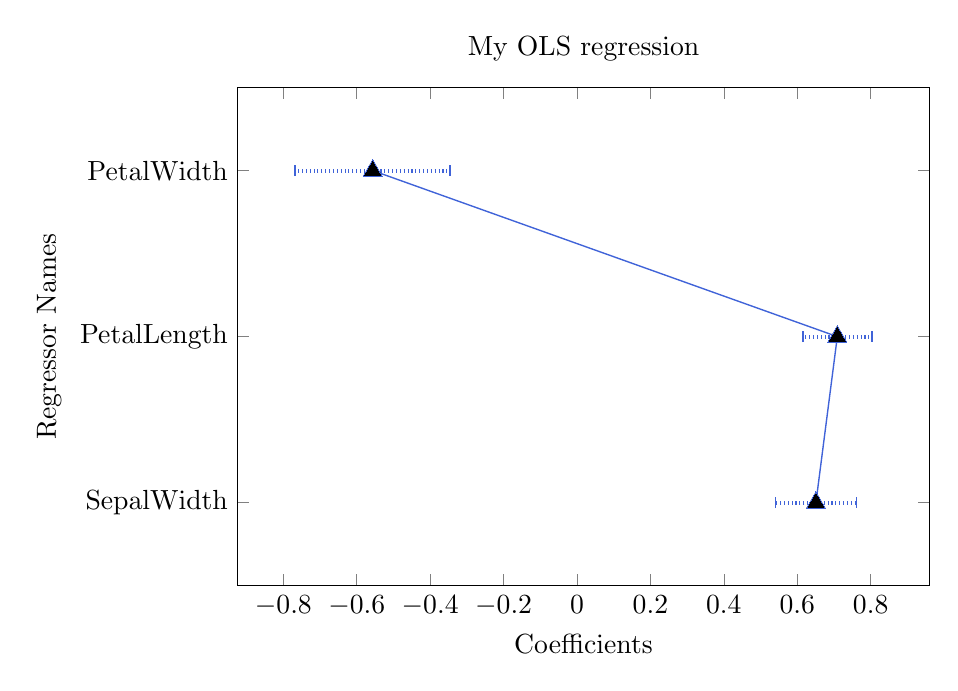
\begin{tikzpicture}
\begin{axis}[title={My OLS regression}, title style={}, xlabel={Coefficients}, xlabel style={}, ylabel={Regressor Names}, ylabel style={}, xticklabel style={}, yticklabel style={}, width={250pt}, height={180pt}, symbolic y coords={SepalWidth,PetalLength,PetalWidth}, ytick={SepalWidth,PetalLength,PetalWidth}, ymin={{[normalized]-0.5}}, ymax={{[normalized]2.5}}, scale only axis]
    \addplot[mark={triangle*}, mark options={mark size={4pt}, line width={0pt}}, error bars/error mark={|}, error bars/error mark options={mark size={2.0pt}, solid, line width={0.6pt}, fill={rgb,255: red, 64; green, 99; blue, 216}, fill opacity={1}, draw={rgb,255: red, 64; green, 99; blue, 216}, draw opacity={1}}, error bars/error bar style={draw={rgb,255: red, 64; green, 99; blue, 216}, draw opacity={1}, densely dotted, line width={1.5pt}}, draw={rgb,255: red, 64; green, 99; blue, 216}, draw opacity={1}, line width={0.5pt}, error bars/x dir={both}, error bars/x explicit]
        coordinates {
            (0.6508371593133089,SepalWidth) +- (0.11032525381627722,0)
            (0.7091319591367299,PetalLength) +- (0.09389069002230775,0)
            (-0.5564826601669999,PetalWidth) +- (0.21113743514223507,0)
        }
        ;
\end{axis}
\end{tikzpicture}
\end{document}
